\section{Bayessche Statistik}
\label{sec:BayesscheStatistik}  

Weerawarana et al. define SOA as an specific architectural style that is concerned with loose coupling and dynamic binding between services \cite{Weera2005}.

In the last years communication between external components whose functionalities are exposed as services has been a hard task when there was not previous agreement on message protocols, data types and encoding, and used middleware technology. Due to the economic and technological growth needed, enterprises had to adapt the \ac{SOA} paradigm in their existing IT Infrastructure. \ac{SOA} provides the needed flexibility by building an architectural style with the following benefits: loose coupling, interoperability, efficiency, and standardization. The W3C group defines SOA as a form of distributed system architecture that is typically characterized by the following properties \cite{w3csoa}:
	\begin{itemize}
		\item Logical view: the service's functionality is exposed, but not its internal logic.
		\item Message orientation: the internal structure of an agent is abstracted.
		\item Description orientation: a service is described by machine-processable meta data.
		\item Granularity: services tend to use a small number of operations with relatively large and complex messages.
		\item Network orientation: Services tend to be oriented toward use over a network.
		\item Platform neutral: Messages are sent in a platform-neutral, standardized format delivered through the interfaces.
	\end{itemize}

\ac{SOA} defines three main roles: requester, provider and broker and the four main operations: publish, find, bind, and invoke. The service provider provides access to services, creates a description of a service and publishes it to the service broker. The service requestor discovers a service by searching through the service descriptions located in the service broker. When the service which best fits to his needs is found, the discovering facility provides the concrete service endpoint and the consumer is responsible for binding to it.  With this information, the requestor can then bind to the concrete service and finally execute a business activity \cite{Weera2005}. The service broker provides support for service registration and binding. 

The main component in a \ac{SOA} is the \ac{ESB}. The functionalities provided by a service bus can simplify the process (publication, discovery, binding, and invocation) and make it more transparent to provide an ease-to-use experience for a Web service based implementation of \ac{SOA} \cite{Weera2005}. Chappel defines its function as an intermediate connection provisioning of service providers with service consumers and thereby ensure decoupling of theses \cite{Chapp2004}. 

\subsection{Definition und Hintergrund}
\subsection{Anwendungsgebiete und Nutzen}
\subsection{Modelle, Parameter und Überzeugungen}
\subsection{Die Wahrscheinlichkeit}
\subsection{Der Satz von Bayes}
The flow of data and information is a key for driving business decisions in IT organizations \cite{Chapp2004}. Furthermore, the interaction between loosely coupled components within an organization or with third party organizations requires distributed systems mechanisms which provide communication support for different protocols, and reliability. SOA has fulfilled this main requirement by providing an integration environment with minimal (or any) integration efforts. 

The \ac{ESB} is the central component in \ac{SOA}. It provides a loosely coupled, event-driven \ac{SOA} with a highly distributed universe of named routing destinations across a multi-protocol message bus \cite{Chapp2004}. An \ac{ESB} provides an abstract decoupling between connected applications by creating logical endpoints which are exposed as services and conform a multi-protocol environment, where routing and data transformation are transparent to the service connected to it. Furthermore, when using an \ac{ESB}, in the first place, services are configured rather than coded, demanding minimal adaptation, implementation and maintenance efforts. The programmer just has to implement the binding to the logical endpoint exposed as a service. In the second place, \ac{ESB} routing is based on a reliable messaging router. Applications don't need to include message system-failure forwarding mechanisms, to know which data formats are needed in the consumed services, or to care about future changes in applications or services the applications interact with. An \ac{ESB} hides the complexity of orchestration between services in business processes. 

Chappel defines the combination of loosely coupled interfaces and asynchronous interactions as a key concept of the bus terminology  \cite{Chapp2004}. A user of the bus can access every service registered in the bus. For this purpose, it implements the \ac{SOA} operations in order to make them transparent to the user who can therefore focus on: plugging to the bus and posting and receiving data from the bus. Furthermore, the \ac{ESB} can form the core of a pervasive grid \cite{Chapp2004}. Services supported by an organization can be organized between the \ac{ESB}s conforming the grid, as well as its access between the organizational departments, and services provided to third party organizations. 

%\begin{figure}[htb]
%	\centering
%		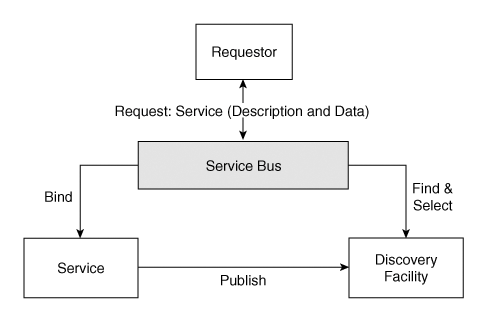
\includegraphics[clip, scale=0.7]{./gfx/servicebus.png}
%	\caption[The Role of the service bus in SOA]{The Role of the service bus in \ac{SOA} \cite{Weera2005} }
%	\label{fig:servicebus}
%\end{figure}

%(see Figure \ref{fig:servicebus})

When receiving a service description (\ac{WSDL}) and data from the service requester, the \ac{ESB} is responsible for selecting the service which best fits to the description requirements, for binding the service requester with the backend service through a route created between the logical endpoints and for making the necessary data transformations to enable the communication between the parts.

As the \ac{ESB} is the central component in \ac{SOA}, and established as integration middleware for services, in this diploma thesis we focus on the required modifications and extensions in the open-source \ac{ESB} Apache ServiceMix 4.3 to provide transparent communication support between the applications and its data located in on-premise databases, or migrated to off-premise data stores. 

\FloatBarrier